\section{External Validation and Failure Analysis}
\label{sec:external}

\paragraph{Setup.}
The unchanged pipeline analysed the UCI-498 incident log~\citep{amaral2018uci498},
a real IT service-desk event log of one organisation, with each final assignment
group of sufficient size treated as an entity: \V{X02b-groups} groups,
\V{X02b-incidents} of \V{X02b-incidents-total} incidents, \V{X02b-events}
investigation-step proxies from work-state events and \V{X02b-reassign}
reassignment-based escalation proxies. The only available outcome is the final
service-level flag; SLA labels were loaded only after SAT-SA's ranking existed and
never entered a submission. \textbf{This is IT incident data, not SOC data.}

\paragraph{Feasibility.}
All \V{X02b-rows-received} submitted rows were accepted
(\V{X02b-rows-rejected} rejected) and every group's analysis completed, with a
median of \V{X02b-analysis-median}\,s per group on SQLite.

\paragraph{Negative result.}
SAT-SA's risk score was not associated with the SLA-miss rate: Spearman
$\rho=\V{X02b-rho-risk}$ (95\% bootstrap \V{X02b-rho-risk-lo} to
\V{X02b-rho-risk-hi}; Table~\ref{tab:external}, Figure~\ref{fig:external}).
Slowest median resolution reached $\rho=\V{X02b-rho-slowest}$
(\V{X02b-rho-slowest-lo} to \V{X02b-rho-slowest-hi}), which is expected because an
SLA miss is a timeliness outcome; reassignment rate reached
\V{X02b-rho-reassign} and volume \V{X02b-rho-volume}. Among the
\V{X02b-relevant} groups in the top SLA-miss quartile, SAT-SA's precision@10\% was
\V{X02b-p10-satsa} (random \V{X02b-p10-random}, slowest resolution
\V{X02b-p10-slowest}), and it needed to review \V{X02b-volume-satsa} groups to
find all of them (slowest resolution: \V{X02b-volume-slowest}).

% Generated by scripts/build_paper_assets.py from satsa-evidence-freeze-v2; do not edit.
% Sources: X02b=EXP-X02b-external-itsm (manifest 036652ed89089874)
\begin{table}[t]
\centering\small
\caption{External IT incident log (X02b): association with the SLA-miss rate over 50 groups of one organization.}
\label{tab:external}
\begin{adjustbox}{max width=\linewidth}
\begin{tabular}{lrr}
\toprule
Score & Spearman $\rho$ & 95\% bootstrap \\
\midrule
Incident volume & \ensuremath{-}0.15 & \ensuremath{-}0.42 to 0.16 \\
Reassignment rate & 0.37 & 0.08 to 0.60 \\
SAT-SA risk score & \ensuremath{-}0.11 & \ensuremath{-}0.42 to 0.21 \\
Slowest median resolution & 0.94 & 0.86 to 0.97 \\
\bottomrule
\end{tabular}
\end{adjustbox}
\par\smallskip\footnotesize Top-quartile precision@10\%: SAT-SA 0.40, random 0.25, slowest resolution 1.00. Not SOC data.
\end{table}


\begin{figure}[t]
\centering
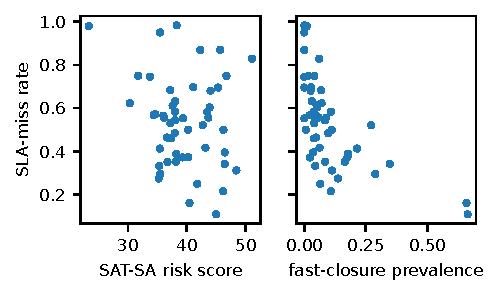
\includegraphics[width=\linewidth]{figures/fig-external.pdf}
\caption{External IT incident log: SAT-SA risk versus SLA-miss rate (left) and
fast-closure prevalence versus SLA-miss rate (right), one point per group
(X02b, X03). Not SOC data.}
\label{fig:external}
\end{figure}

\paragraph{Failure analysis.}
A diagnostic analysis (X03) on the same data changed no detector, threshold or
weight. It attributes the result to four causes.
\emph{(1) Construct mismatch (primary).} The prevalence of fast closures was
negatively associated with SLA misses ($\rho=\V{X03-rho-fast}$,
\V{X03-rho-fast-lo} to \V{X03-rho-fast-hi}): on a service desk fast resolution is
the goal, whereas SAT-SA treats fast closure of security alerts as possible skipped
investigation. The execution-gap dimension, which this signal drives, correlated at
$\V{X03-rho-execgap}$ (\V{X03-rho-execgap-lo} to \V{X03-rho-execgap-hi}).
\emph{(2) Existence-rule saturation.} In total, \V{X03-saturated} detector
families fired for every group, although their input conditions varied widely---cases without any
step \V{X03-cases-min} to \V{X03-cases-max} of cases, medium-or-higher alerts with
fewer than two steps \V{X03-alerts-min} to \V{X03-alerts-max}. A rule that fires on
``at least one'' qualifying record cannot discriminate submissions with thousands
of tickets, and the fusion adds near-constant amounts for these families because it
ignores prevalence. Risk still took \V{X03-risk-distinct} distinct values and was
unrelated to volume ($\rho=\V{X03-risk-vs-volume}$).
\emph{(3) Unavailable constructs.} Of the \V{CODE-dimensions} risk dimensions,
\V{X03-zero-dims} had no input data; investigation steps and escalations are proxies (state changes and
reassignments), and monitoring coverage is unavailable.
\emph{(4) An adapter artifact.} The log has no step notes; the adapter submits
empty notes, which satisfy the repeated-investigation note rule in
\V{X03-note-rule} groups.

The analysis found no temporal or label defect: risk and label cover the same
incidents and period; only \V{X03-other-group} of \V{X03-missed} SLA misses
occurred while another group held the ticket; and reassigned incidents missed
more often (\V{X03-reassigned-miss} versus \V{X03-notreassigned-miss}),
consistent with the positive reassignment association. The one pipeline defect
found---ingestion totals recorded as null---affected bookkeeping only; its fix
produced X02b with identical analytical outputs.

\paragraph{Decision and interpretation.}
No risk-model change was made. A change that raised the correlation with SLA
misses would optimise SAT-SA toward a timeliness construct it does not claim to
measure, using the evaluation data for tuning. We therefore read X02b and X03 as
\emph{feasibility and construct-validity evidence rather than external-effectiveness
validation}: the unchanged pipeline processed real workflow data, and on data
whose outcome measures a different construct and lacks investigation, escalation
and coverage semantics, SAT-SA's supervisory signals did not transfer. The
prevalence-blind fusion of existence rules is a design limitation in SAT-SA's own
domain; addressing it needs SOC development data held out from evaluation.
